\section{Evaluation}
This section first presents the experimental setups and then assesses \system from the following aspects:
\begin{itemize}
    \item Does \system improve query throughput while maintaining recall when plugging into existing ANNS systems? (Section~6.2)
    \item How much additional memory does \system introduce? (Section~6.3)
    \item How important is the validation gate for balancing throughput improvement and recall preservation? (Section~6.4)
    \item How do the key storage and retrieval parameters affect performance? (Section~6.5)
    \item How does \system behave under different numbers of threads? (Section~6.6)
\end{itemize}
\subsection{Experimental Setup}
\noindent \textbf{Test-bed.} Experiments are conducted on a Linux Server (Ubuntu 22.04) with two Intel Xeon Gold 5117 CPUs (each with 14 cores, 2.00GHz) and 512GB memory.

\noindent \textbf{Baselines.} We evaluate \system on CANDOR-Bench~\cite{Wang202627} by deploying it on three representative ANNS systems and comparing their performance with and without \system under the same dynamic benchmark protocol.
(1) HNSW~\cite{Malkov2020824}, one of the most widely-used ANNS systems;
(2) SymphonyQG~\cite{Gou2025}, a recent static ANNS system that combines graph index with RabitQ quantization technique; and 
(3) Wolverine~\cite{Liu20252268}, a dynamic ANNS system designed for online updates.
We denote the corresponding \system-enabled variants as HNSW-\system, SymphonyQG-\system, and Wolverine-\system.


\noindent \textbf{Datasets.} We choose four million-scale datasets, \texttt{SIFT}, \texttt{OpenImages}, \texttt{Msong}, and \texttt{Glove}.
These datasets cover image, audio, and text embeddings with different dimensionalities. 
Table~\ref{tab:eval-datasets} summarizes their statistics. 

\begin{table}[t]
    \centering
    \caption{Datasets used in evaluation.}
    \label{tab:eval-datasets}
    \begin{tabular}{lcccc}
        \toprule
        Dataset & Type & Dimension & DataSize & QuerySize \\
        \midrule
        SIFT & Image &128 & 1,000,000 & 10,000 \\
        OpenImages & Image & 512 & 1,000,000 & 10,000 \\
        Msong & Audio & 420 & 992,272 & 200 \\
        Glove & Text & 100 &  1,192,514 & 200 \\
        \bottomrule
    \end{tabular}
\end{table}

\noindent \textbf{Metrics.} We use end-to-end query throughput and Recall@$k$ as the primary metrics. 
Throughput is measured in queries per second (QPS), computed as the number of executed queries divided by the total post-update query processing time.
Unless otherwise stated, we report Recall@10 against the exact nearest-neighbor ground truth.

\noindent \textbf{Parameters.} For graph-based backends, the graph out-degree is set to $M=16$; the construction beam width is 
set to \textit{efConstruction}$=120$; and the default search beam width is set to \textit{efSearch}$=80$. 
These settings provide a balanced recall--latency tradeoff on million-scale datasets.

\noindent \textbf{Evaluation Protocol.} For each dataset, we use half of the vectors to build the initial index and treat the remaining vectors as dynamic updates, which are applied in batches of 10,000 vectors.
After each update batch, we execute the corresponding query batch and record QPS and Recall@10, following the round-based update-then-query execution model of CANDOR-Bench.
Each experiment is repeated three times, and we report the average result.

\subsection{QPS Performance and Recall}

\begin{figure*}[t]
    \centering
    \subfloat[SIFT]{
        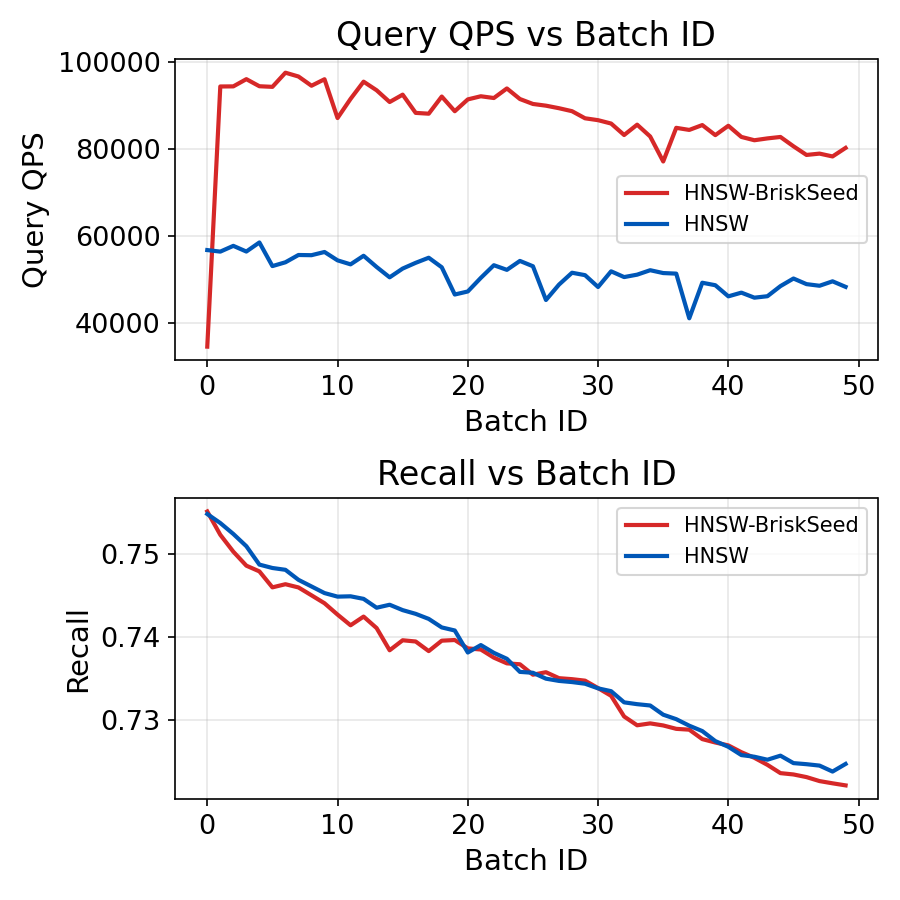
\includegraphics[width=0.31\textwidth]{figures/sift.png}
    }\hfill
    \subfloat[Msong]{
        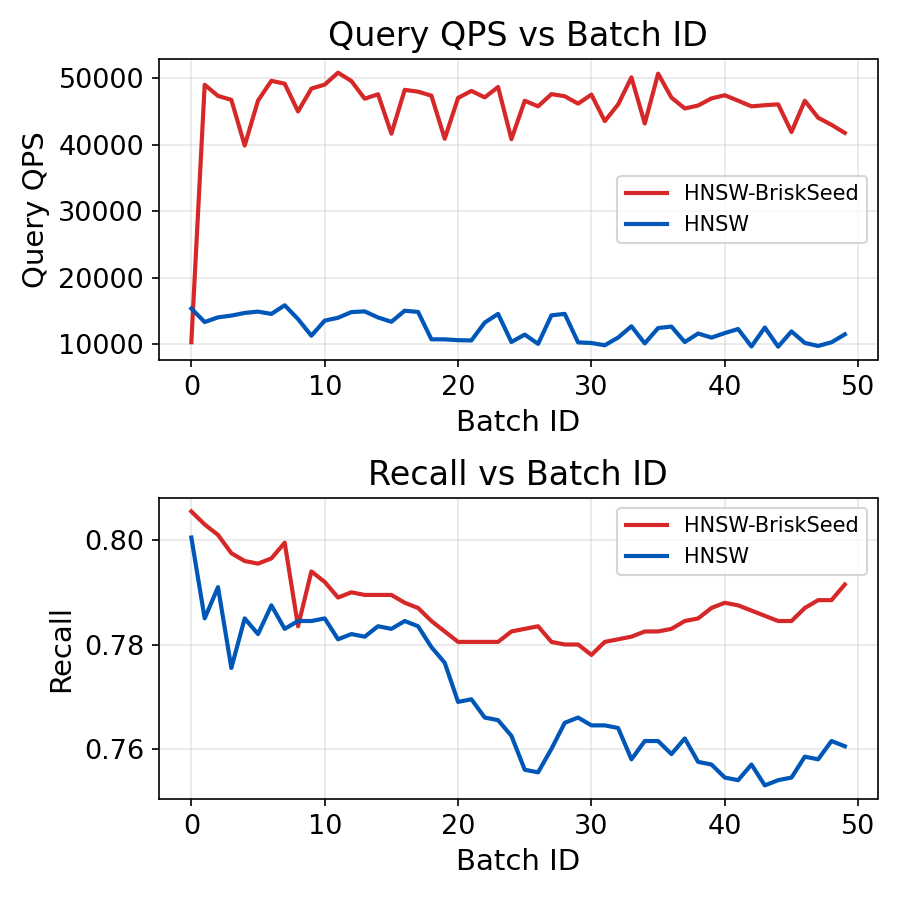
\includegraphics[width=0.31\textwidth]{figures/msong.png}
    }\hfill
    \subfloat[Glove]{
        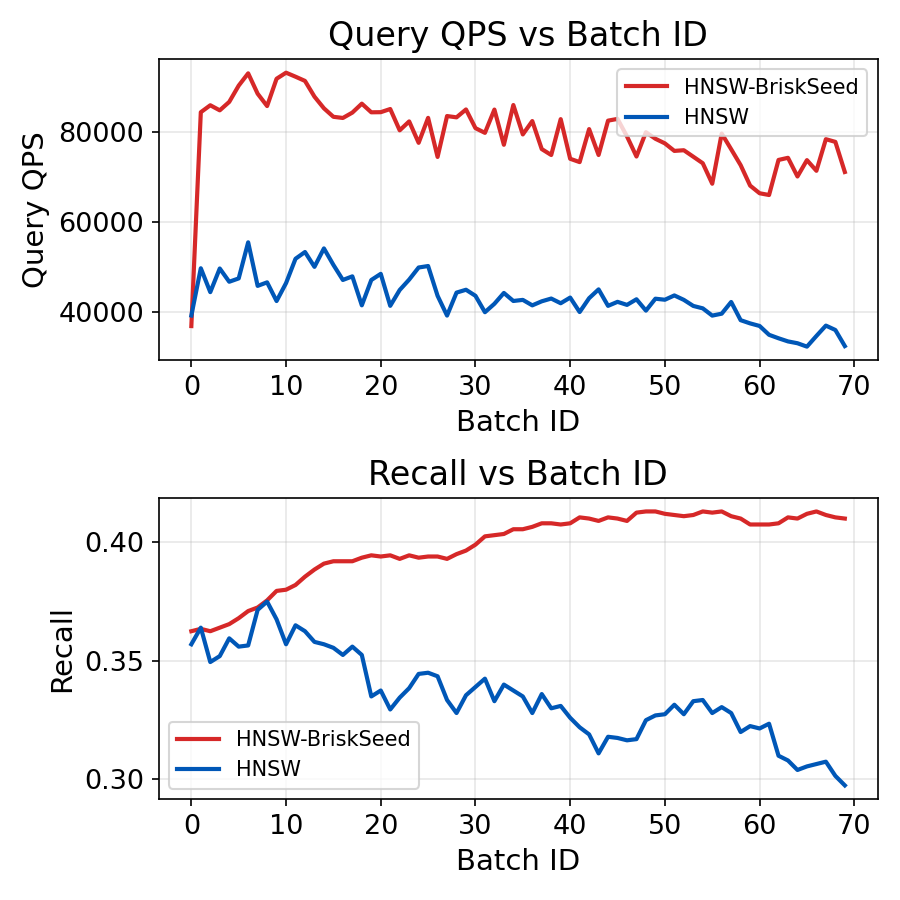
\includegraphics[width=0.31\textwidth]{figures/glove.png}
    }
    \caption{QPS and Recall comparison between the baseline and \system on three datasets.}
    \label{fig:qps-recall-three-datasets}
\end{figure*}

\subsection{Memory Usage}

\subsection{Ablation Study}

\subsection{Parameter Study}

\subsection{Scaling-up Study}